\chapter{Testing}

\section{MPU}
In order to test the memory partition mapping, for an amount of space given, we use a non-specific initial
 pointer representing the begining of the memory free space, specific sizes for each partition and we
  write in each memory position the number of the partition that is ocupied with. In the end we print the
   whole memory avaiable for the test and confirm if the space given for each is enough and if they are
    allocated in the right place.\\
  If the amount of memory needed is bigger than the memory given a segmentation fault occurs.\\
 The tests cover the different partition memory distribuitions and sizes in memory, for the 3 cases of not
  having 1, 2 or  3 subregions used by the main partition of the region. For that we used 5 partitions, with
   specific memory requirements, in order to test the different memory alloctions combinations.\\
  The results printed showed us that the new sizes and subregions distribution allow us to have the less 
  spare memory possible, comparing with the theoretical calculations.\\
\begin{figure}[H]
\centering
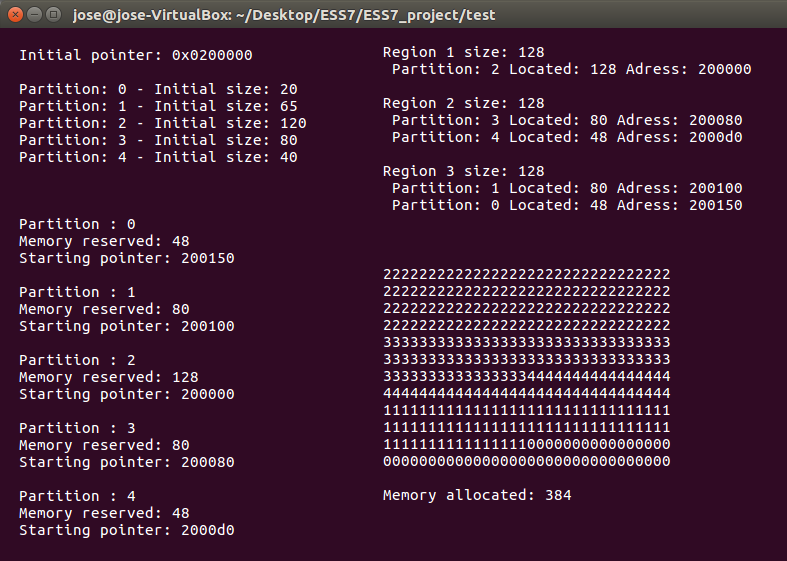
\includegraphics[width=15cm]{mpu_test.png}
\captionof{figure}{Terminal displaying the results}
\label{fig:simple_system}
\end{figure}

\section{XML validation}

Currently there is no validation of the XML file. 
The XML is currently prone to human error when manually 
adding to the file, also does it does not prevent elements 
not compliant with the schema being written. 
\\


\section{Scheduler}

\section{\arinc{} specification - Part 3}
In order to test a system for compliance with \arinc{}, Aeronautical
Radio Inc., the authors of the standard provide a conformity test
specification. This comes as a separate document, as a part of the
\arinc{} specification:
\begin{itemize}
	\item\textbf{Part 0}Introduction to ARINC 653
	\item\textbf{Part 1}Required services. This includes system services,
	data structures and functional behaviour.
	\item\textbf{Part 2}Extended services. For example file handling or external events
	\item\textbf{Part 3}\textbf{Conformity test}
	\item\textbf{Part 4}Subset Services
	\item\textbf{Part 5}Core Software Recommended Capabilities
\end{itemize}

Basically, software developers should use this to test the compliance with
Part 1 of the standard. The extended services (Part 2), are not being
tested. This could be done in the future phases of the \OSname{} OS in order
to demonstrate the compliance of the APEX behavior.

\section{Message passing}

\section{The evil partition}